\documentclass{beamer}
\usetheme{metropolis}
\usepackage{graphicx}
\usepackage{amsmath}
\usepackage{tcolorbox}
\title{College Writing Seminar (INTD100): Week 6 Notes}
\author{Jordan Hanson}
\institute{Whittier College Department of Physics and Astronomy}

\begin{document}
\maketitle

\section{Summary}

\begin{frame}{Summary}
\small
\textbf{Week 6}: \textit{The Laboratory Report II:} The thread
\begin{enumerate}
\item Exercises: Identify breaks in the thread of logic.
\item Exercises: Write passages that preserve the thread, transitions and mini-outlines.
\item Homework/Asynchronous: Rearrange a passage to patch the thread together
\item Work on final essay
\end{enumerate}
Exploration topic: climate science and climate skepticism.
\end{frame}

\section{Writing about a DIY Experiment}

\begin{frame}{Writing about a DIY Experiment}
\small
\textbf{\alert{You are in your house anyways, so why not experiment?}} Write down the process for completing an experiment in your house.  Examples are listed below.  Research how to accomplish your chosen project.  Write down a cohesive set of instructions in passive voice with technically accurate language.  \textbf{Exchange documents with a partner and attempt to perform the procedure they outline.}
\begin{enumerate}
\item Create a compass with a needle, magnetizing magnet, cork, and bowl of water
\item Measure the acceleration of gravity from the period of a pendulum
\item Create a ``homopolar'' motor with a copper wire and a magnet
\item Create a lemon battery
\item Measure the acceleration of gravity by timing the fall of an object
\end{enumerate}
\end{frame}

\section{The Thread of Logic}

\begin{frame}{The Thread of Logic}
Consider the following two outlines:
\begin{figure}
\centering
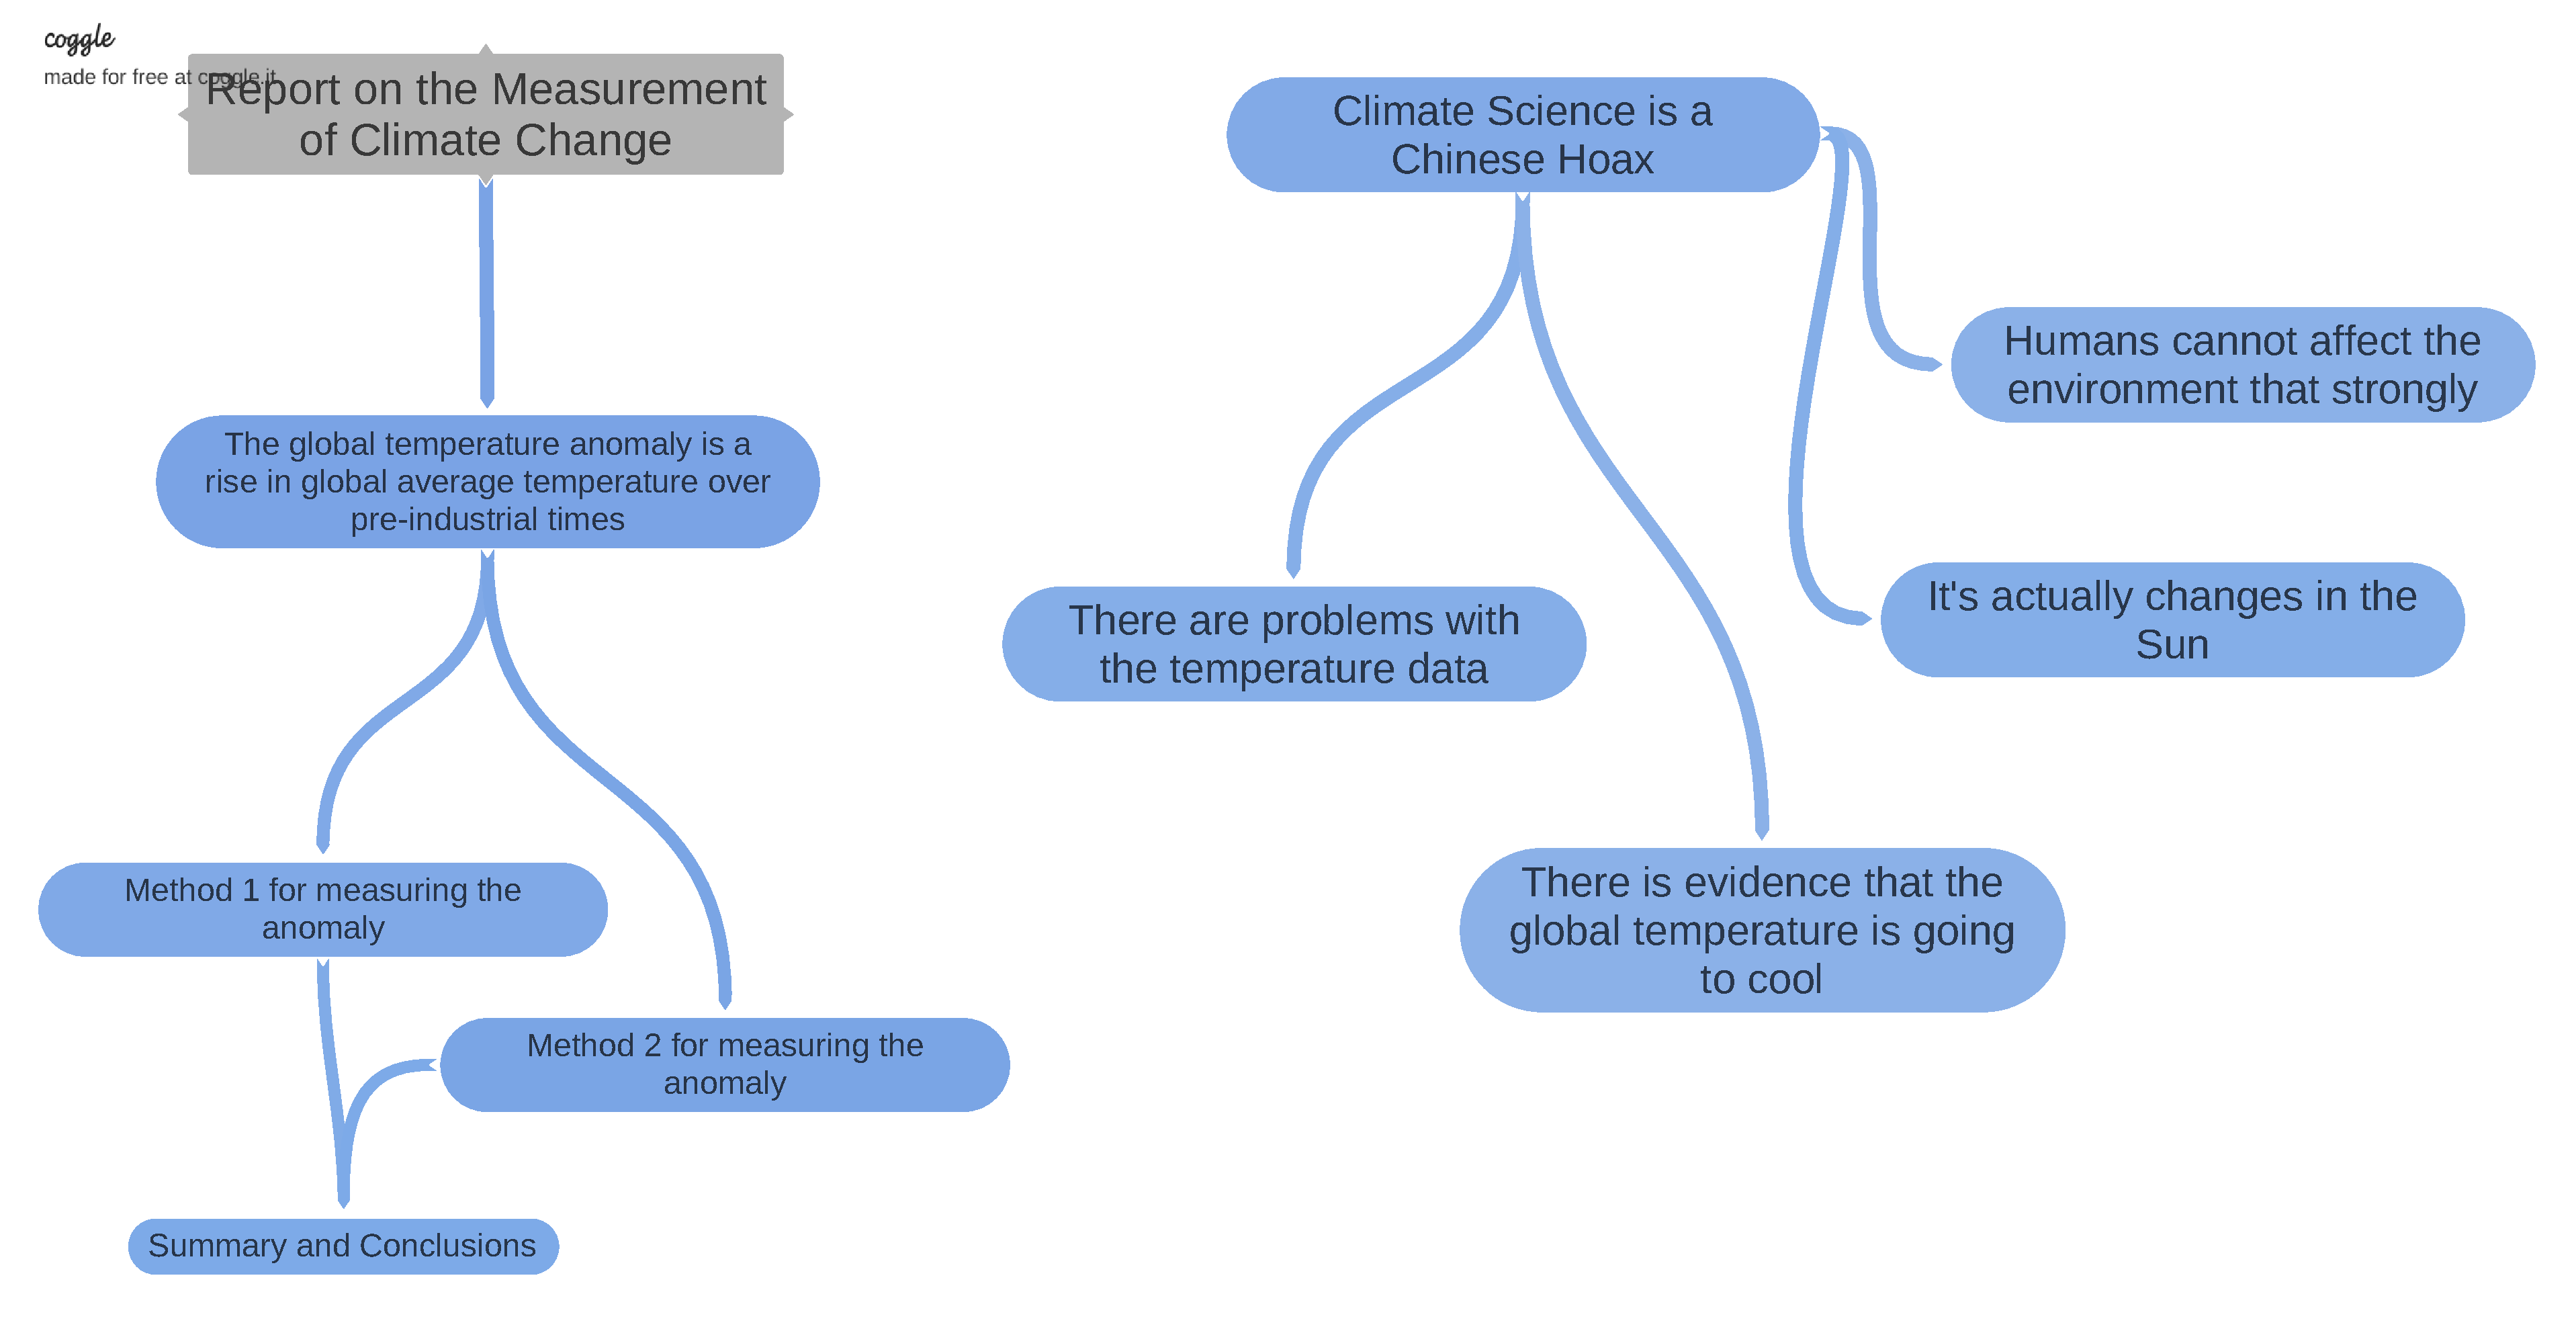
\includegraphics[width=0.9\textwidth]{figures/climate.pdf}
\caption{\label{fig:climate} Two examples of mind maps that have different threads. (Left) a linear thread.  (Right) a more amorphous thread.}
\end{figure}
\end{frame}

\begin{frame}{The Thread of Logic}
Several protips for preserving the thread of logic:
\begin{enumerate}
\item Provide a \textit{mini-outline.} (next slide).
\item Remember that your reader likely thinks \textit{linearly.}  Topic A, \textit{then}, topic B, \textit{then} topic C ...
\item Use transition sentences.
\end{enumerate}
\end{frame}

\begin{frame}{The Thread of Logic}
\alert{Mini-outlines are useful for establishing the thread.}
\begin{enumerate}
\item Go to Moodle and download the PDF file ``AntennaSimulationPaper''
\item Read the first two pages, including the abstract
\item Where is the mini-outline?
\end{enumerate}
\end{frame}

\begin{frame}{The Thread of Logic}
\small
\begin{enumerate}
\item Numerical simulation applied to electromagnetic scattering problems represents a very broad and multifaceted field.
\item In this fast-growing background, the use and the development of numerical software for electromagnetic simulation follow two main directions.
\item However, in both situations, the knowledge of the existing open-source possibilities is often scarce.
\item Moreover, it is very rare that more than one academic institution work together for the practical development of open-source simulation packages ...
\item We only believe that a proper knowledge of the existing open-source alternatives can be very useful for researchers working in this field.
\end{enumerate}
\end{frame}

\begin{frame}{The Thread of Logic}
\small
\begin{enumerate}
\item We only believe that a proper knowledge of the existing open-source alternatives can be very useful for researchers working in this field.
\item The goal of the present paper is to review open-source software in electromagnetic scattering simulation, and in particular to identify possible open-source programs that can be fruitfully used in the design of antennas and its workflow.
\end{enumerate}
\end{frame}

\section{Review of Asynchronous Activity}

\begin{frame}{Review of Asynchronous Activity}
In breakout sessions, answer the following questions together:
\begin{enumerate}
\item (True or false): The conclusion of the literature review regarding climate science is that $97.1$ percent of peer-reviewed scientific results agree that anthropogenic climate change is real.  \textit{How would you modify or clarify this statement?}
\item Describe how the authors collected all the papers they analyzed.  How many papers made it in to the study?
\item Any scientific study or analysis is subject to potential statistical errors or biases.  How was this literature review constructed so as to mitigate potential biases or errors?
\end{enumerate}
\end{frame}

\section{Topic Sentences, Transitions}

\begin{frame}{Topic Sentences, Transitions}
\alert{This week's asynchronous activity} involved topic sentences.  Hopefully, reading the topic sentences gave you a clue as to the thread of the article. \\ 
\begin{enumerate}
\item Take turns sharing your map of the climate science literature review in breakout discussions (4 people)
\item Having seen the maps of others, how can you modify yours to be more \textit{linear?}
\item Recall: linear in this context means that the next idea follows from the current one.
\end{enumerate}
\end{frame}

\begin{frame}{The Thread of Logic}
\begin{figure}
\centering
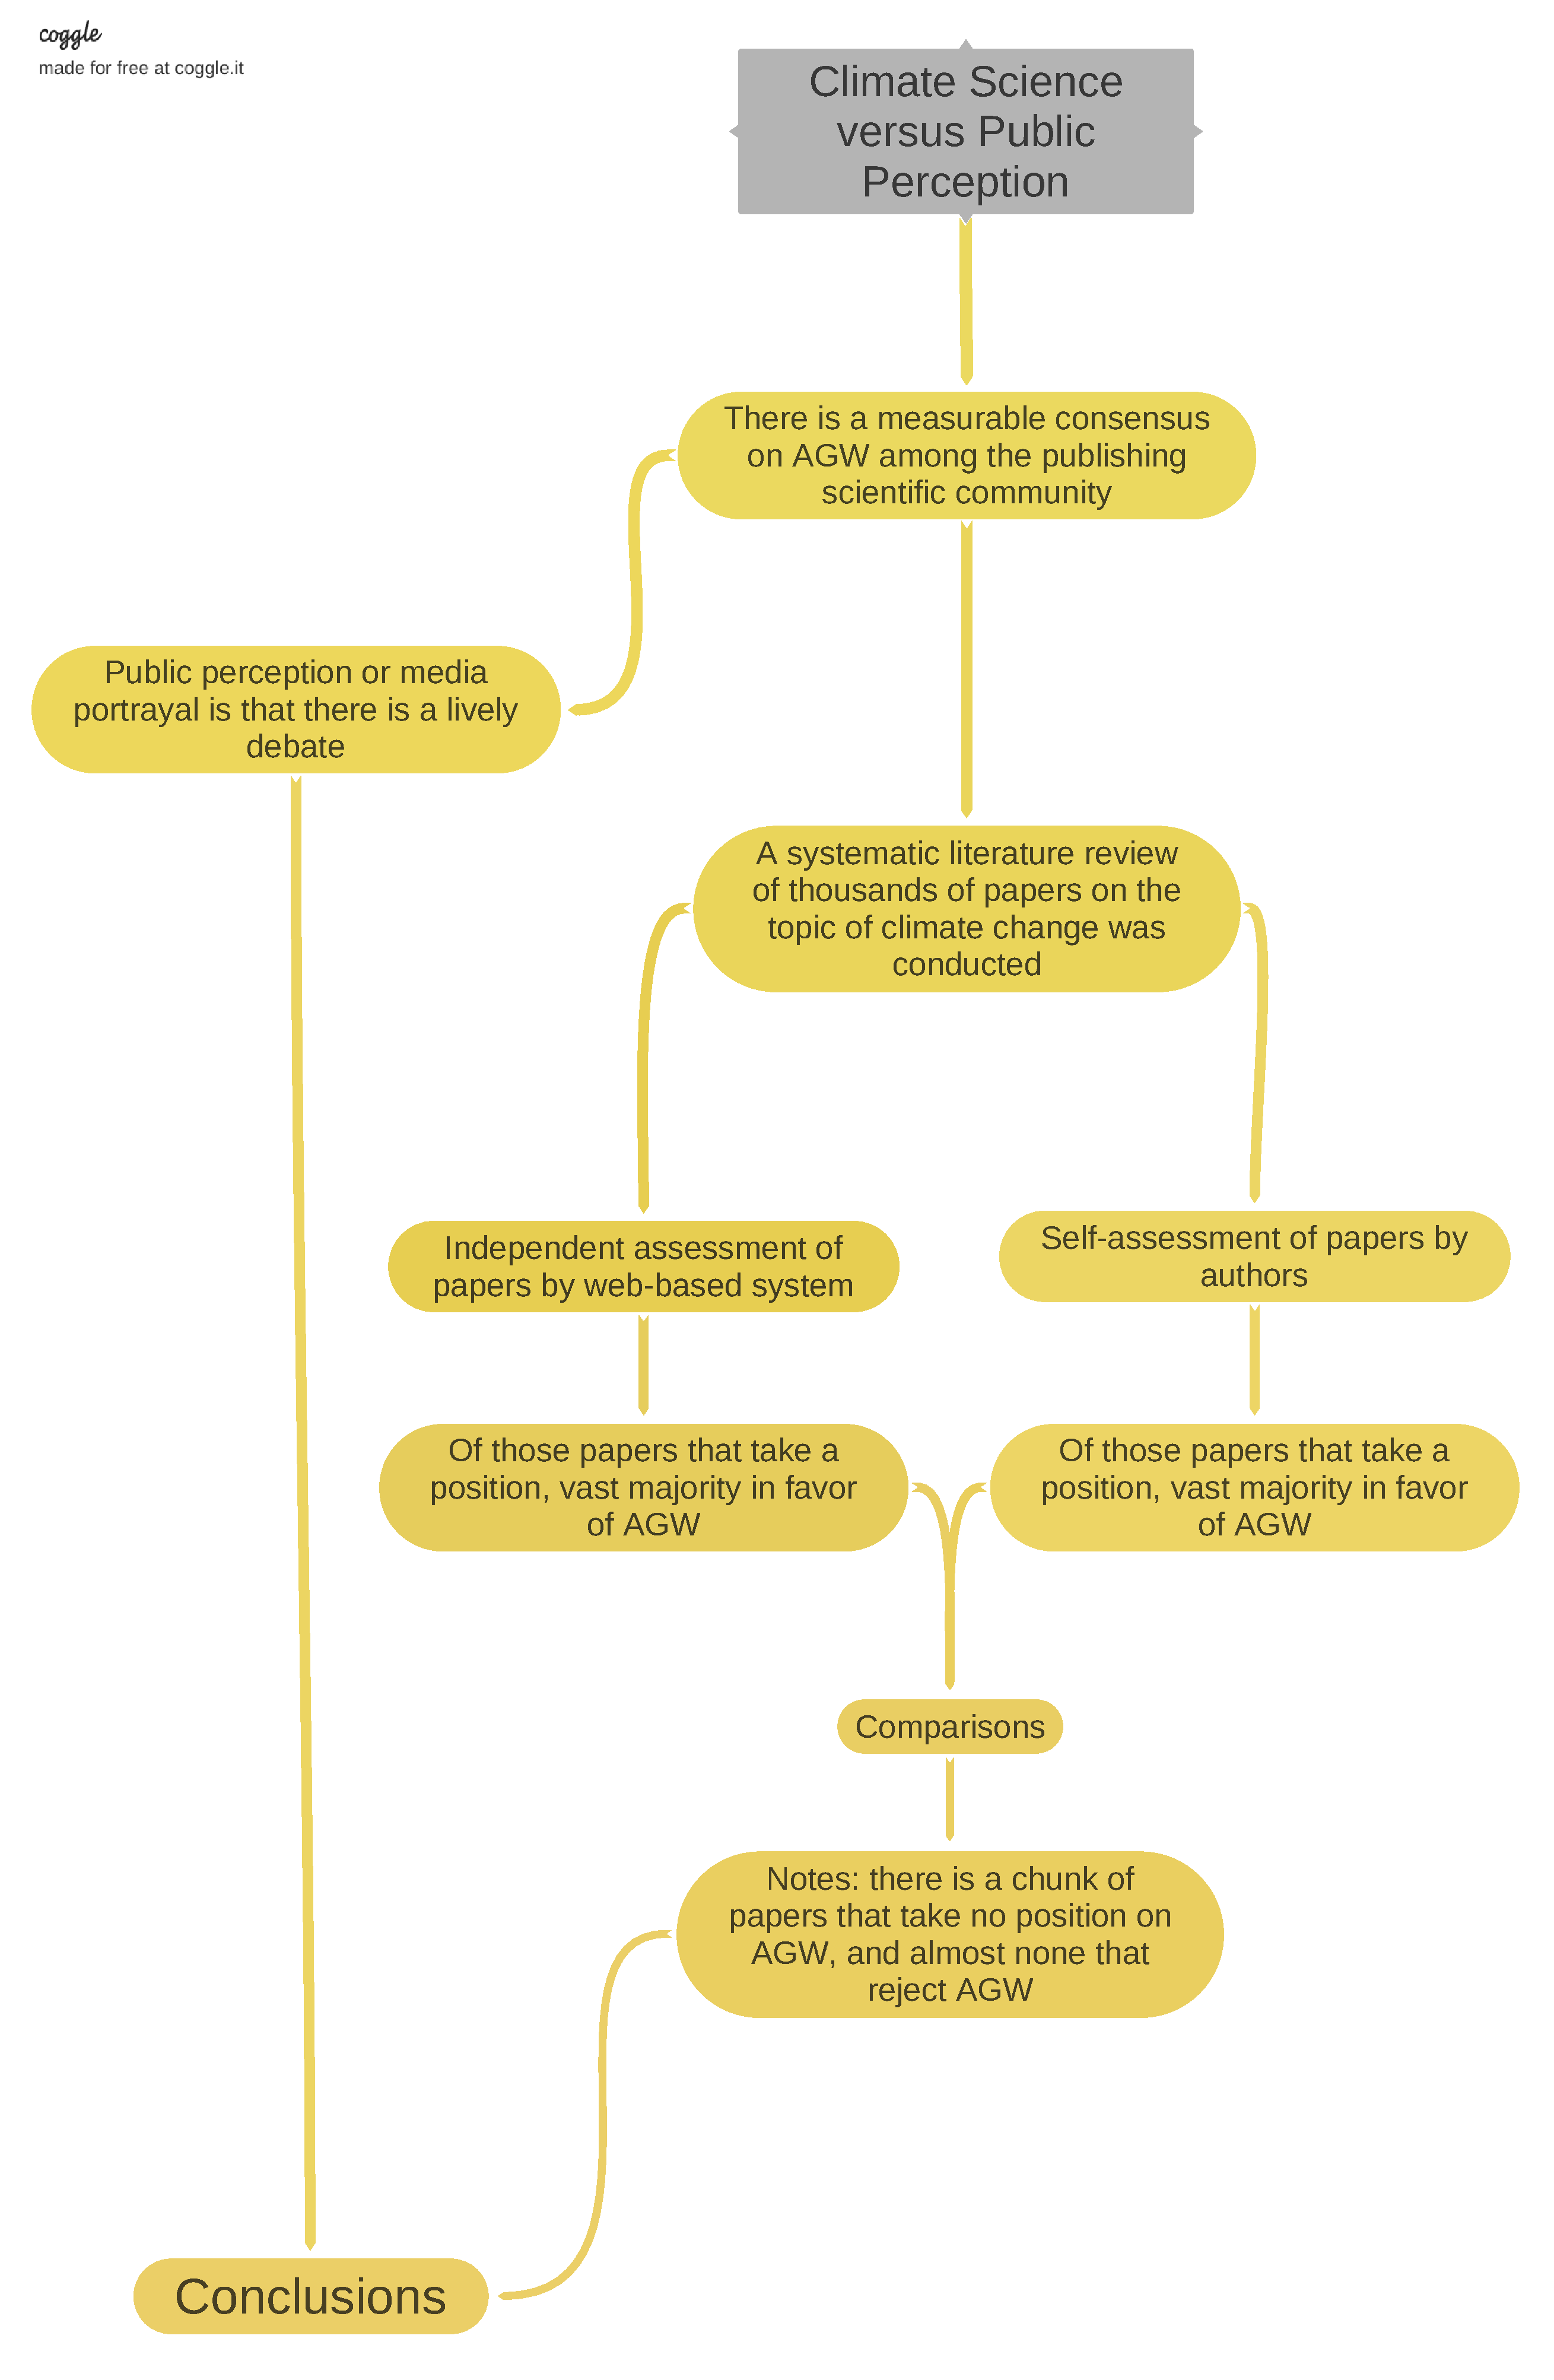
\includegraphics[width=0.4\textwidth]{figures/climate2.pdf}
\caption{\label{fig:climate2} An example of a linear map of the thread from the climate science literature review.}
\end{figure}
\end{frame}

\section{Conclusion}

\begin{frame}{Summary}
\small
\textbf{Week 6}: \textit{The Laboratory Report II:} The thread
\begin{enumerate}
\item Exercises: Identify breaks in the thread of logic.
\item Exercises: Write passages that preserve the thread, transitions and mini-outlines.
\item Homework/Asynchronous: Rearrange a passage to patch the thread together
\item Work on final essay
\end{enumerate}
Exploration topic: climate science and climate skepticism.
\end{frame}

\section{Thank You}

\begin{frame}{Thank You}
\begin{figure}
\centering
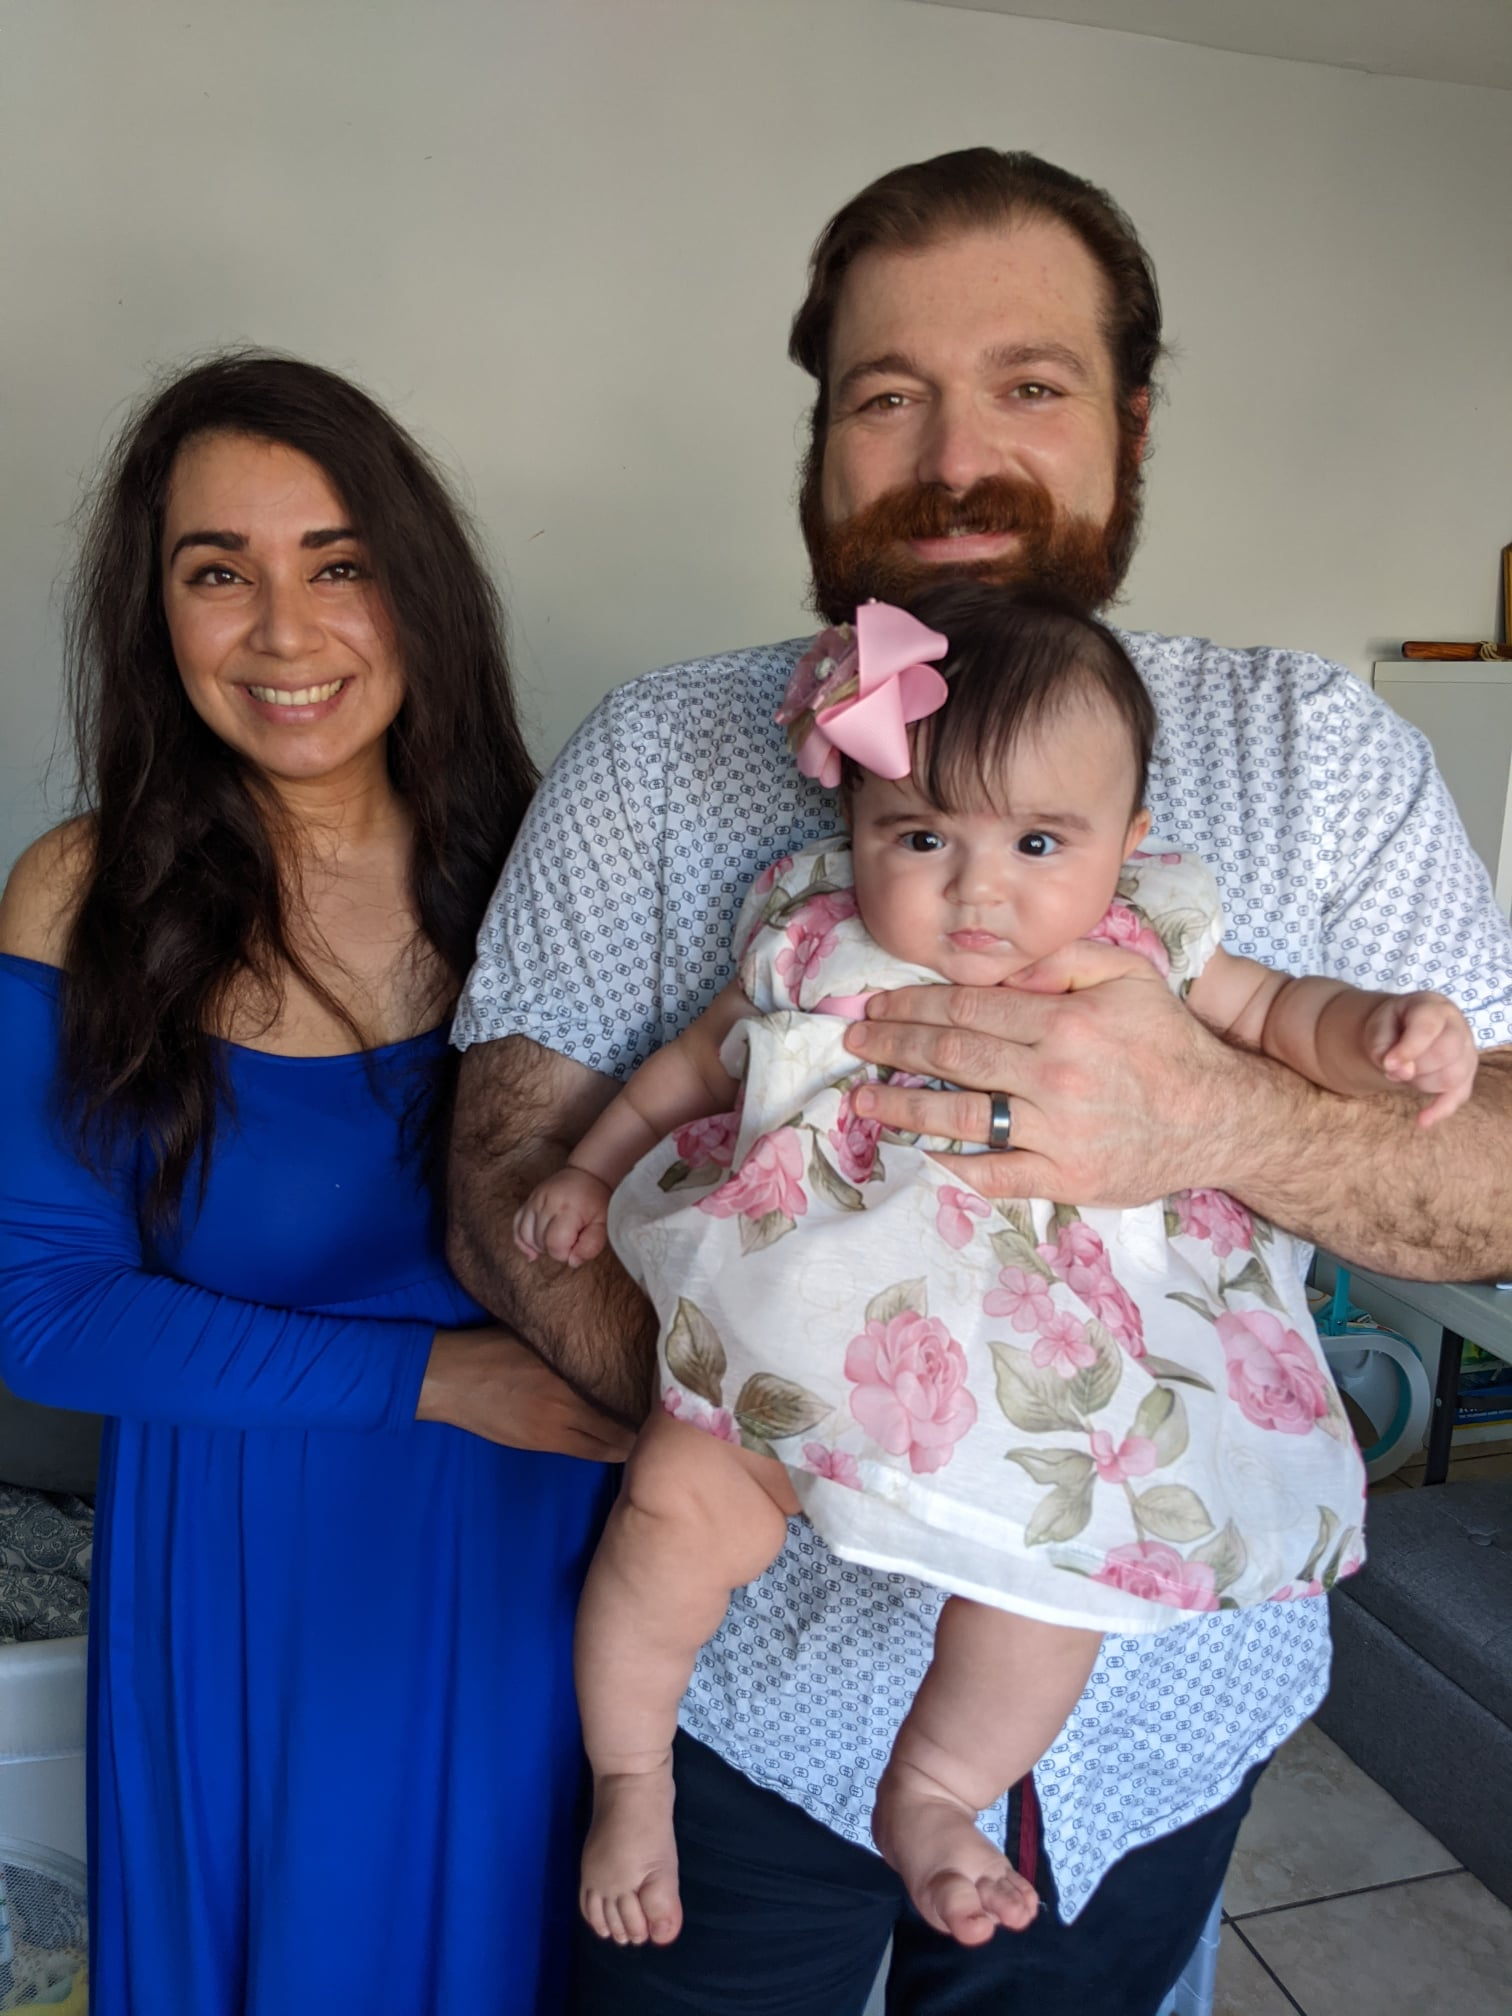
\includegraphics[width=0.42\textwidth]{figures/fam1.jpg}
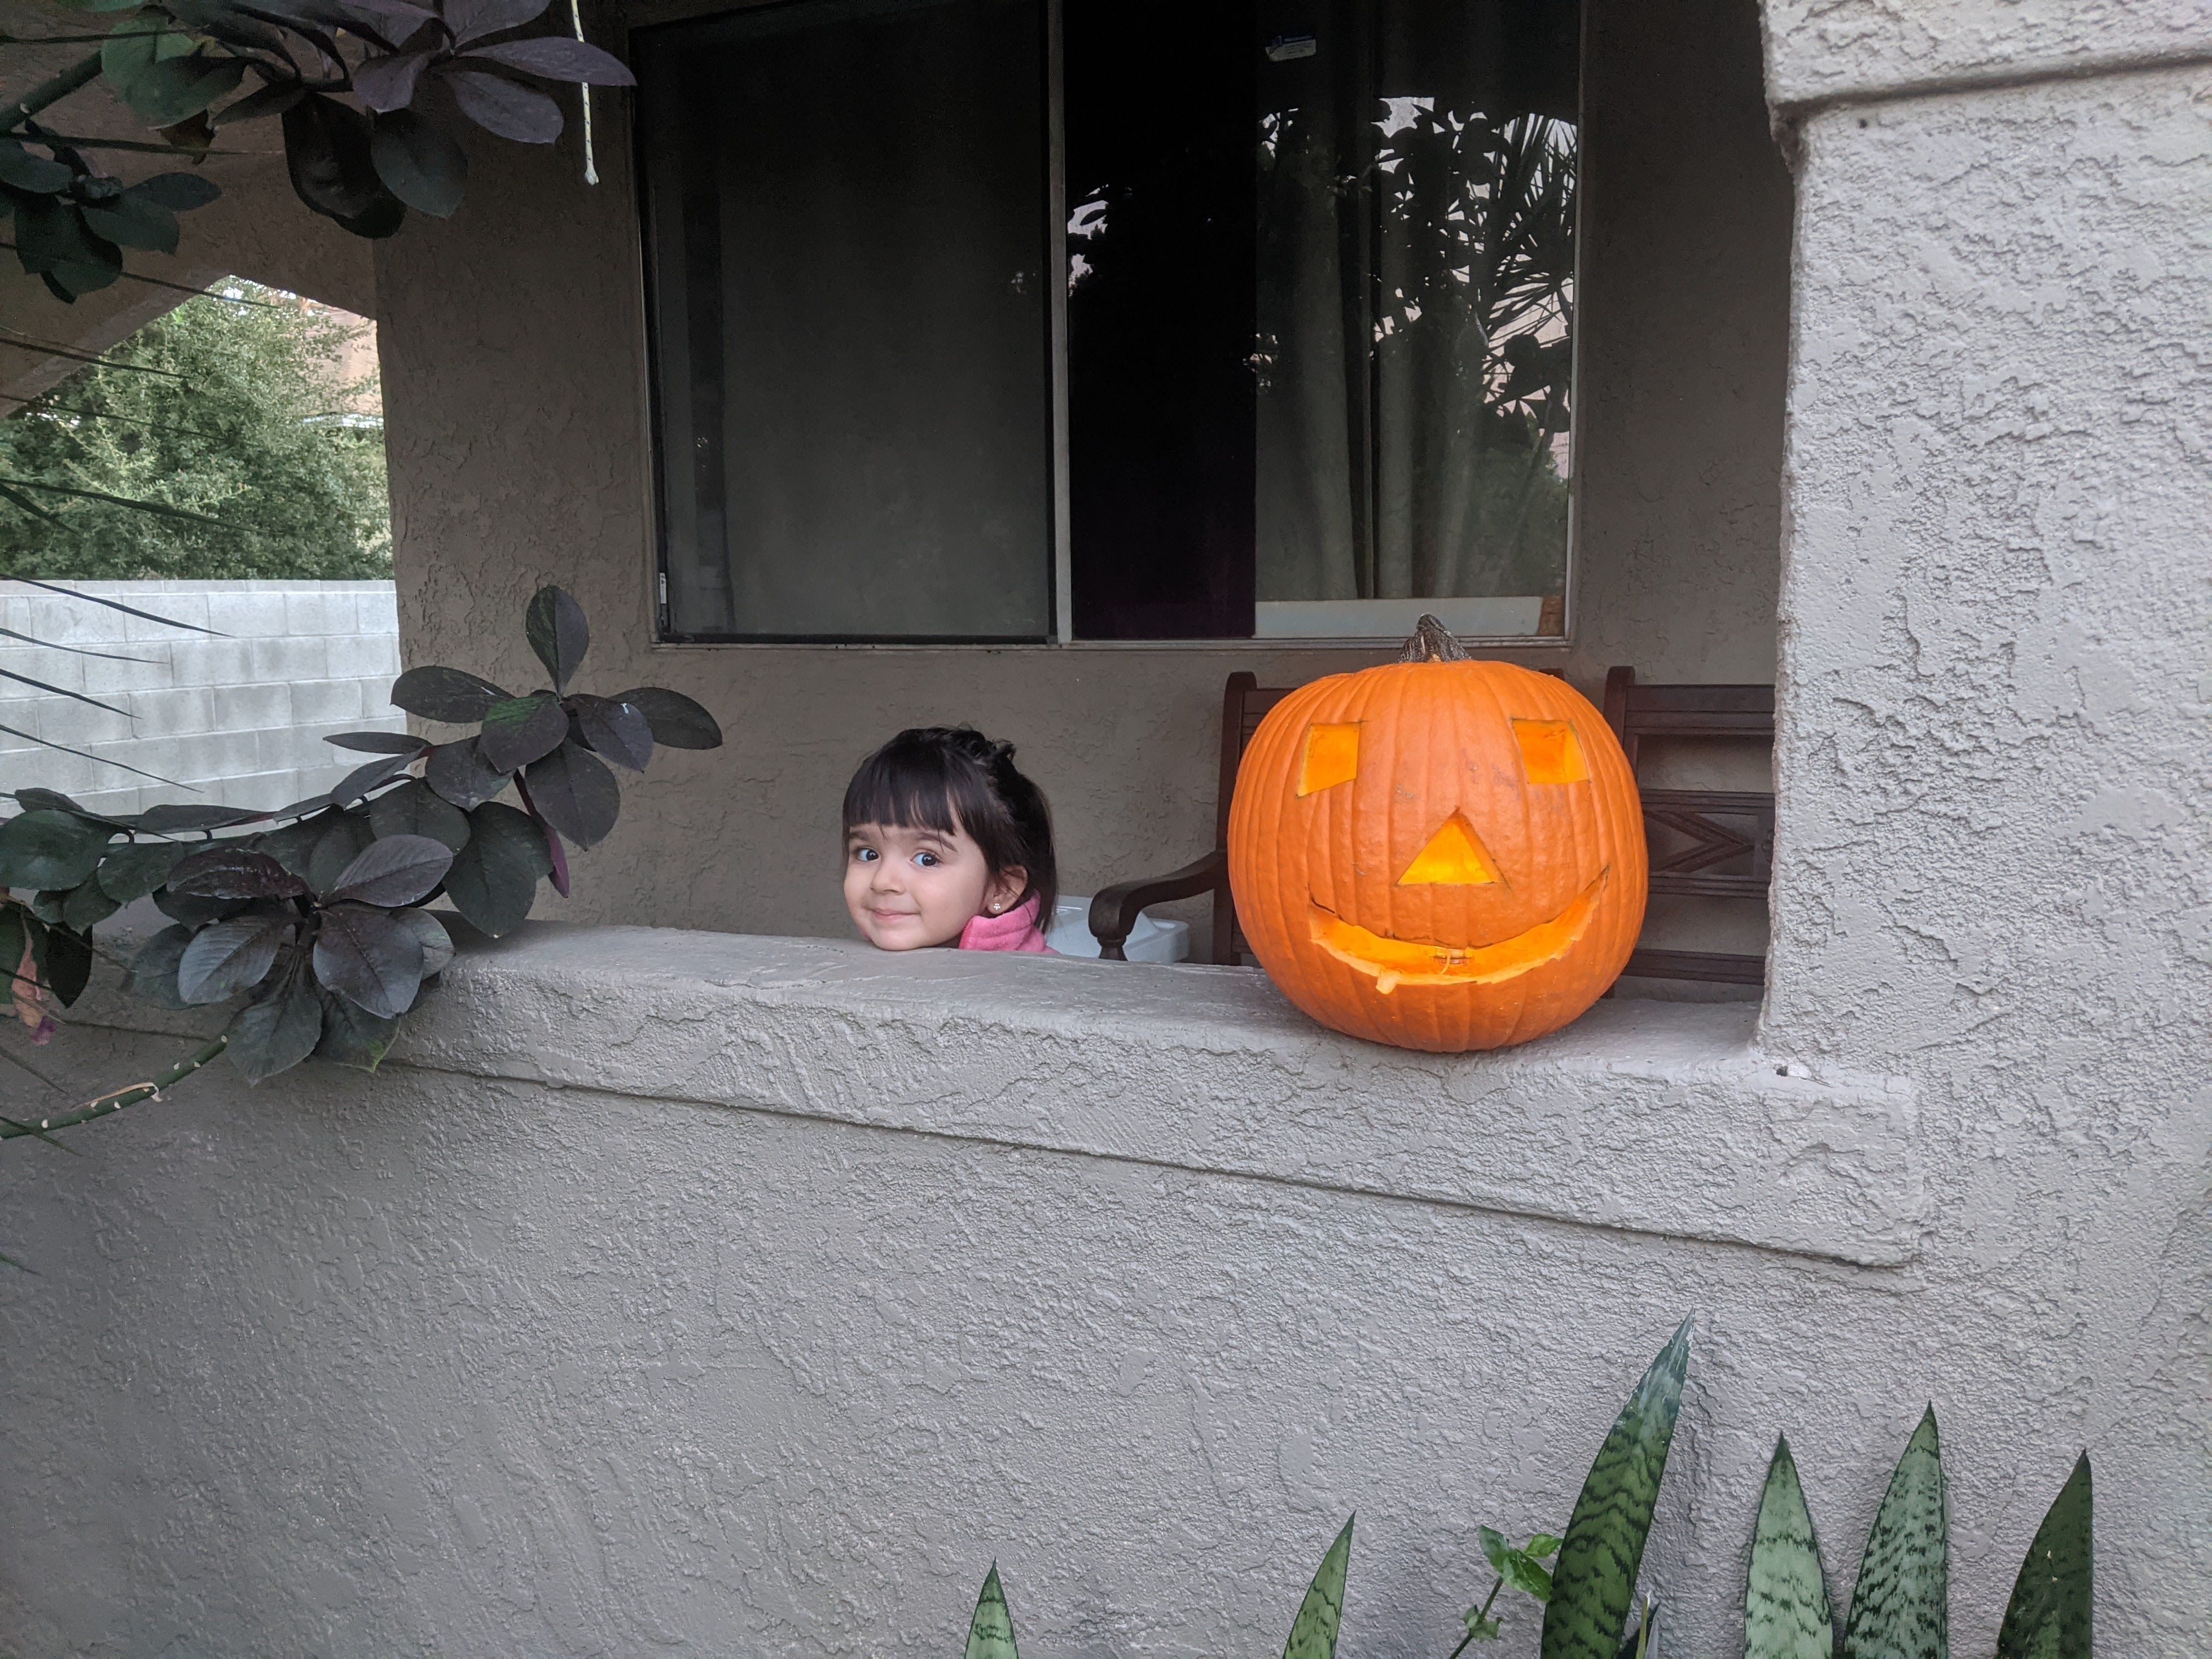
\includegraphics[width=0.42\textwidth]{figures/fam2.jpg}
\caption{\label{fig:fams} We are grateful to you and Whittier College.  Thank you for your hard work this Module, and hang tough.  We will get through this together.}
\end{figure}
\end{frame}

\end{document}
